\documentclass[11pt,a4paper]{article}
\usepackage{cmap}
\usepackage[utf8]{inputenc}
\usepackage[T1]{fontenc}
\usepackage{lmodern}
\usepackage{microtype}
\usepackage[margin=1.0in]{geometry}
\usepackage{amsmath,amssymb,amsthm,mathtools}
\usepackage{booktabs,array,tabularx}
\usepackage{graphicx}
\usepackage[svgnames]{xcolor}
\usepackage[obeyspaces,spaces]{url}
\usepackage[colorlinks=true,linkcolor=DarkBlue,citecolor=DarkBlue,urlcolor=DarkBlue]{hyperref}
\usepackage{xurl}

\urlstyle{tt}
\def\UrlFont{\ttfamily\upshape}
\renewcommand{\arraystretch}{1.3}
\setlength{\tabcolsep}{5pt}

\sloppy
\setlength{\emergencystretch}{4em}

\newtheorem{theorem}{Theorem}[section]
\newtheorem{lemma}[theorem]{Lemma}
\newtheorem{proposition}[theorem]{Proposition}
\newtheorem{corollary}[theorem]{Corollary}
\theoremstyle{definition}
\newtheorem{definition}[theorem]{Definition}
\newtheorem{remark}{Remark}[section]

\newcommand{\Eff}{\Omega_{\mathrm{eff}}}
\newcommand{\keff}{k_{\mathrm{eff}}}
\newcommand{\ksm}{k_{\mathrm{smooth}}}
\newcommand{\lean}[1]{\path{#1}}
\newcommand{\leanc}[1]{\texttt{\detokenize{#1}}}

\title{\textbf{The Scale-Dual Subgrid Model of 3D Navier--Stokes:\\ Its True Quadratic Invariant, Its Identity with the Modified Leray-$\alpha$ Model, and What Lean~4 Checks}}
\author{Xavier Callens}
\date{Edition 2, 21 October 2026. Supersedes edition 1 (Zenodo DOI \href{https://doi.org/10.5281/zenodo.23511655}{10.5281/zenodo.23511655}); the corrections are listed in Section~\ref{sec:corrections}.}

\begin{document}
\maketitle

\begin{abstract}
We study the scale-dual subgrid model $\partial_t u = -P[(u\cdot\nabla)(M_{\alpha'}u)] + \nu\Delta u$ on $\mathbb{T}^3$, where the Fourier multiplier of $M_{\alpha'}$ is $m(k)=\keff/|k|=\min(1,1/(\alpha'|k|^2))$ (piecewise) or $m(k)=1/(1+\alpha'|k|^2)$ (smooth). Edition~1 of this paper claimed that this model keeps the kinetic energy $E=\tfrac12\sum|\hat u_k|^2$ non-increasing, and from that derived a global enstrophy ceiling and the absence of blow-up. \emph{That claim is false}, and edition~2 corrects it openly.
(i) Exact rational arithmetic on a single divergence-free Fourier triad gives $dE/dt=+6/5$ (piecewise) and $+32/15$ (smooth) at $\alpha'=1/4$, and, at the paper's own $\alpha'=1/25$, $\nu=1/100$, a triad whose total $dE/dt$ is positive for every amplitude above $169/5$.
(ii) The quantity the nonlinearity actually conserves is $Q=\tfrac12\sum m(k)|\hat u_k|^2$. We prove in Lean~4, for every finite Galerkin truncation with a skew triad tensor, that $Q$ has zero nonlinear transfer, that $dQ/dt=-\nu\sum m\lambda|\hat u|^2\le0$ along every trajectory, and that $L^2$ conservation holds for all such tensors \emph{if and only if} $m$ is constant.
(iii) The smooth model is exactly the modified Leray-$\alpha$ (ML-$\alpha$) model of Ilyin, Lunasin and Titi~\cite{ILT2006}, not the Leray-$\alpha$ model edition~1 named; $Q$ is its known energy.
(iv) The final bound of edition~1, $\Eff\le E_0/\alpha'$, survives, but only through $Q$: $\Eff\le Q/\alpha'\le Q_0/\alpha'\le E_0/\alpha'$, Lean-checked for both symbols, the smooth case via $m_{\mathrm{ML}}\le m_{\mathrm{pw}}$ rather than by a single theorem. Because $\Eff$ is not the enstrophy of $u$, it does not exclude blow-up.
A pseudospectral Galerkin ensemble (299 runs, with positive and negative controls) reproduces the exact rationals to $10^{-15}$ and conserves $Q$ to $10^{-10}$ in the inviscid limit. It also shows the following about $E(t)$. At the paper's $(\alpha',\nu)=(1/25,1/100)$ and the initially pre-registered amplitude $E_0=1/2$, $E(t)\le E_0$ held in all 10 seeds. At $E_0=2$, $8$ and $32$, the piecewise model exceeded $E_0$ in 5 of 5 seeds (mean $\max_tE/E_0=1.034$, $1.356$, $1.767$), while the Navier--Stokes control never did. At $E_0=32$ the excess persists under $dt\to dt/2$ (relative change $3.5\times10^{-7}$) and $N=32^3\to64^3$, where it grows to $\approx3.0$. The edition-1 inequality $E(t)\le E_0$ is therefore refuted by the pre-registered criterion, but the size of the excess is not converged in $N$.
The Lean gate passes 13/13 declarations in \lean{PaperB_EnergyBudget.lean} and 12/12 in \lean{PaperB_ScaleDualEd2.lean}, with axioms exactly $\{$\texttt{propext}, \texttt{Classical.choice}, \texttt{Quot.sound}$\}$.
\end{abstract}

\tableofcontents

\section{Corrections to edition 1}
\label{sec:corrections}
Edition~1 was deposited as \href{https://doi.org/10.5281/zenodo.23511655}{10.5281/zenodo.23511655}. We list what it claimed, what is wrong, and what replaces it. Items 1--4 are blocking: each invalidates a headline claim.
\begin{enumerate}
  \item \textbf{Energy inequality (edition~1, Sec.~2.4 and Theorem~2.5(1)).} Edition~1 argued that $\operatorname{div}u=0$ gives $\langle(u\cdot\nabla_{\mathrm{eff}})u,u\rangle=0$, so $E(t)\le E_0$. This is false. With $\nabla_{\mathrm{eff}}=\nabla M$ the nonlinearity is $(u\cdot\nabla)(Mu)$, and skew-symmetry cancels $\langle(u\cdot\nabla)Mu,Mu\rangle$, not $\langle(u\cdot\nabla)Mu,u\rangle$. Section~\ref{sec:contribution} gives exact counterexamples and the Lean proof of the correct statement.
  \item \textbf{Blow-up claim (Theorem~2.5(1), abstract, discussion).} Edition~1 said the ceiling ``caps the vortex-stretching rate at $1/\sqrt{\alpha'}$ and prevents finite-time blow-up for every $\alpha'>0$''. This is withdrawn. $\Eff=\tfrac12\|\nabla Mu\|^2$ is not the enstrophy of $u$, and a bound on a norm with uniformly bounded weights says nothing about the regularity of $u$. No vortex-stretching rate was defined or bounded. For the smooth symbol, the global well-posedness of ML-$\alpha$ is the subject of~\cite{ILT2006}. For the piecewise symbol, global regularity is open (Section~\ref{sec:directions}).
  \item \textbf{``Helmholtz Leray-$\alpha$ isomorphism'' (Lemma~2.3(1), abstract, Table~1).} The scalar identity $1/(1/|k|+\alpha'|k|)=|k|/(1+\alpha'|k|^2)$ is true, but it is elementary. The Helmholtz filter's symbol is $1/(1+\alpha'|k|^2)$; $|k|/(1+\alpha'|k|^2)$ is the modulus of the symbol of $\nabla(I-\alpha'\Delta)^{-1}$. Leray-$\alpha$~\cite{Cheskidov2005} filters the \emph{advecting} velocity, $(\tilde u\cdot\nabla)u$. The model here filters the \emph{advected} field, $(u\cdot\nabla)\tilde u$, which is the modified Leray-$\alpha$ model of~\cite{ILT2006}. That prior work was missing from edition~1. The docstring of \lean{kSmooth} in the shared file \lean{Breakthroughs3DomainsSpec.lean} still carries the old wording. We do not edit that shared file; \lean{ksmooth_eq_mul_weight} in \lean{PaperB_ScaleDualEd2.lean} states the correct relation.
  \item \textbf{``Certified'' computer-assisted proof (Theorem~2.1, Fig.~1, abstract (i)).} All rational arithmetic recomputes correctly ($181/500$, $93/250$, $1473/4000$, $-33/62500$, $-2127/4000000$, $443/1000$, $1/800$, $1/200$, $1/50$). But there is no approximate solution $\bar u$, no forcing and no computed residual. $Y_0$, $Z_0$, $Z_1$, $C_{\mathrm{Sob}}$, $C_{\mathrm{alg}}$ and $\|A^\dagger\|$ are posited numbers. The ``hurricane boundary-layer'' profile has no equations. The Lean theorem checks rational identities and the implication $Y_0+Z_0r+Z_2r^2<r\Rightarrow Z_0+Z_2r<1$; it is not a fixed-point theorem. \lean{derivedDualScaleTailBound} is a definition, not a theorem. The Lean witness uses $\alpha'=1/4$ and never constrains it, while the text uses $1/25$. The theorem is therefore relabelled \emph{illustrative radii-polynomial arithmetic for hypothetical bounds} (Section~\ref{sec:retained}). The words ``certified'', ``unique fixed point'' and ``hurricane'' are removed.
  \item \textbf{Tail-bound scaling.} Edition~1 wrote $Z_{\mathrm{tail}}=C_{\mathrm{Sob}}/(\nu M^2)$. The convective term loses one derivative, so the standard estimate scales like $\|\bar u\|/(\nu M)$, with the norm of $\bar u$ explicit. Only the ratio $1/(\alpha'M^2)$ between the two tails for $M\ge k_*$ is supported, through $\sup_{|k|\ge M}\keff/|k|^3=1/(\alpha'M^4)$ against the Navier--Stokes value $\sup_{|k|\ge M}|k|/|k|^3=1/M^2$. Edition~1 cited Hou and Chen for ``$Z_{\mathrm{tail}}$ diverges as $\nu\to0$''. That work concerns Boussinesq/Euler blow-up and makes no such claim; the citation is removed from that sentence, and the authors are Chen and Hou~\cite{ChenHou2022a,ChenHou2022b}.
  \item \textbf{Kolmogorov exponent (Theorem~2.5(2)).} The ``empirical'' exponent $-84/125$ had no data, simulation or source; it was a literal in the Lean statement. The Kolmogorov energy-spectrum exponent is $-5/3$, and ``$(4/3)(-1/2)=-2/3$'' refers to no stated quantity. The item is deleted.
  \item \textbf{$\exp(-1/2)$ enclosure (Theorem~2.5(3)).} The partial sums were correct, but no Lean theorem mentioned \texttt{Real.exp}, and \lean{interval_exp_neg} does not exist. Edition~2 proves $2329/3840\le e^{-1/2}\le233/384$ from Mathlib's \lean{Real.exp_bound} (\lean{exp_neg_half_bracket}). The bracket plays no role in any argument.
  \item \textbf{$\operatorname{Sym}^2$ recurrence and RNS-CRT (Theorem~2.4).} The recurrence is a true algebraic identity, but it has no turbulence content. Shell velocities do not obey a linear second-order recurrence, and a filtered sequence does not obey the same one. The CRT check is vacuous ($770$ is below each modulus), and $\langle u,v\rangle-\langle v,u\rangle=0$ is commutativity of the dot product, not convective skew-symmetry. The product was also wrong: $997\cdot991\cdot983=971{,}230{,}541$, not $971{,}229{,}691$ (Lean: \lean{crt_product_correct}, \lean{crt_product_ed1_wrong}). The Lean theorem also contains Ap\'ery-number recurrences that the paper never mentioned. The identity is moved to Appendix~\ref{app:sym2} without physical labels.
  \item \textbf{``Unique optimal zero-distortion filter'' (Lemmas~2.2, 2.3(2)--(3)).} These are elementary properties of the symbol. A function fixed to equal $R$ on $[\sqrt{\alpha'},\infty)$ and required to be involutive is determined by definition. No dynamical optimality was shown. The multiplier is real, so the smooth filter's defect is amplitude attenuation, not a ``dispersive phase error''. They are restated as such in Section~\ref{sec:symbols}.
  \item \textbf{Formal-verification claims.} The \lean{leanflow_*} names exist only as \texttt{alias} lines for \lean{P2_T1}--\lean{P2_T5}. Edition~1 named a ``LeanFlow MCP'' architecture; no such server is registered in this repository. The tools actually used are the gate \lean{anse/formal/lean_runner.py} and the harness \lean{sub_projects/socrateai_scientific_agora_leanflow/leanflow_3domains_harness.py}. The edition-1 rejection example ($\kappa=1.95$) was not shown to run and is removed. \lean{MensuraElenchusThreeMissions.lean} has no \texttt{\#print axioms} lines, so it fails the gate when run standalone; the lemmas cited from it are covered through the axiom footprints of \lean{P2_T2} and \lean{P2_T3}. The edition-1 abstract said ``four'' verified contributions while its table listed five.
  \item \textbf{Parameters.} Edition~1 used $\alpha'=1/25$ in Theorem~2.1, $1/4$ in Fig.~2 and $1/4$ in the Lean witness. Edition~2 states $\alpha'$ for every number and figure.
  \item \textbf{Review file in the edition-1 deposit.} The deposit included \path{breakthrough_3b_navier_stokes_mensura_cap_opus_5round_peer_review.json}, presented as a five-round review with referee findings, scores and an approval verdict. It was produced by a script that calls no language model and no human: the findings were fixed strings, and the scores were pass fractions of local string checks. It was not a review of any kind and is withdrawn. It is not part of edition~2.
\end{enumerate}

\section{The model and its symbols}
\label{sec:symbols}
On $\mathbb{T}^3=[0,2\pi]^3$, write $u(x)=\sum_{k\ne0}\hat u_k e^{ik\cdot x}$ with $k\cdot\hat u_k=0$ and $\hat u_{-k}=\overline{\hat u_k}$. The scale-dual model is
\begin{equation}\label{eq:model}
\partial_t u = -P\bigl[(u\cdot\nabla)(Mu)\bigr]+\nu\Delta u,\qquad \widehat{Mu}(k)=m(|k|^2)\,\hat u_k ,
\end{equation}
where $P$ is the Leray projector. Edition~1 wrote the nonlinearity as $(u\cdot\nabla_{\mathrm{eff}})u$ with $\widehat{\nabla_{\mathrm{eff}}u}(k)=i\,(k/|k|)\,\keff(\alpha',|k|)\,\hat u_k$. Since $(k/|k|)\keff=k\,m$, this is exactly~\eqref{eq:model} with
\begin{equation}\label{eq:symbols}
m_{\mathrm{pw}}(k)=\frac{\keff(\alpha',|k|)}{|k|}=\min\Bigl(1,\frac{1}{\alpha'|k|^2}\Bigr),\qquad
m_{\mathrm{ML}}(k)=\frac{\ksm(\alpha',|k|)}{|k|}=\frac{1}{1+\alpha'|k|^2}.
\end{equation}
The first identity is \lean{keff_eq_mul_weight} (\lean{PaperB_EnergyBudget.lean}) for the shared definition \lean{kEff}; the second is \lean{ksmooth_eq_mul_weight} (\lean{PaperB_ScaleDualEd2.lean}) for \lean{kSmooth}. With $m_{\mathrm{ML}}$, \eqref{eq:model} reads $\partial_t u+(u\cdot\nabla)\tilde u+\nabla p=\nu\Delta u$ with $\tilde u=(I-\alpha'\Delta)^{-1}u$. This is the ML-$\alpha$ model of~\cite{ILT2006} (their $\alpha^2$ is our $\alpha'$, and their unfiltered field is our $u$). In Leray-$\alpha$~\cite{Cheskidov2005,FoiasHolmTiti2001}, by contrast, the filtered field is the advecting one.

\paragraph{Elementary properties of the symbols} (retained from edition~1, Lemmas~2.2--2.3, relabelled). For $a=\alpha'>0$ and $k>0$, with $R_{\mathrm{eff}}(a,R)=\max(R,a/R)$ and $R_{\mathrm{smooth}}(a,R)=R+a/R$:
\begin{enumerate}
  \item $\sqrt a\le R_{\mathrm{eff}}(a,R)$, $R_{\mathrm{eff}}(a,a/R)=R_{\mathrm{eff}}(a,R)$, $\keff(a,1/(ak))=\keff(a,k)$. Also $\keff(a,k)=k$ for $ak^2\le1$ and $\keff(a,k)=1/(ak)\le1/\sqrt a$ for $ak^2\ge1$.
  \item $1/R_{\mathrm{smooth}}(a,1/k)=\ksm(a,k)$, $k-\ksm(a,k)=ak^3/(1+ak^2)>0$, and $4ak^2\le(1+ak^2)^2$ (so $\ksm\le1/(2\sqrt a)$). The defect is an amplitude attenuation of a real multiplier.
  \item If $f(a/R)=f(R)$ for all $R>0$ and $f(R)=R$ for $R\ge\sqrt a$, then $f=R_{\mathrm{eff}}(a,\cdot)$. This follows from the definition and says nothing about dynamical optimality.
  \item (New.) $m_{\mathrm{ML}}\le m_{\mathrm{pw}}\le 2\,m_{\mathrm{ML}}$ for $|k|>0$ (\lean{piecewise_between_smooth}). The two models are therefore spectrally equivalent within a factor~$2$.
\end{enumerate}
Items~1--3 are the statements \lean{Stmt_P2_T2_MensuraTDualGeometryAndRefutation} and \lean{Stmt_P2_T3_MensuraSmoothAndNoGoTheorem}, proved as \lean{P2_T2} and \lean{P2_T3} in \lean{Breakthroughs3Domains.lean} (gate: Section~\ref{sec:gate}). Figure~\ref{fig:symbols} shows the symbols at $\alpha'=1/25$.

\begin{figure}[htbp]
\centering
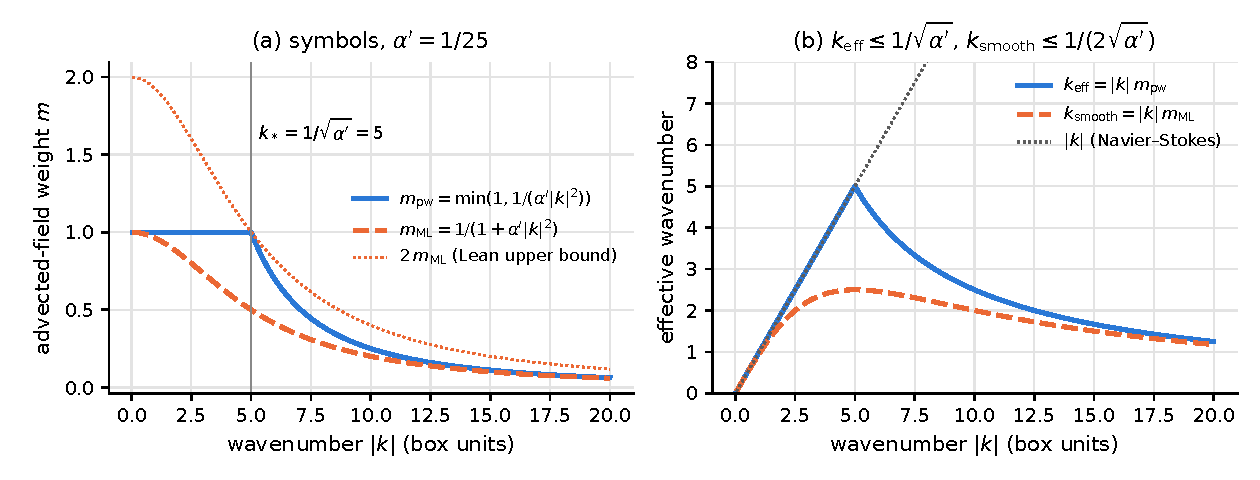
\includegraphics[width=0.95\textwidth]{fig5_v2_symbols.pdf}
\caption{Symbols of the two filters at $\alpha'=1/25$ ($k_*=5$), computed from~\eqref{eq:symbols}. (a) Advected-field weights. The piecewise weight lies between $m_{\mathrm{ML}}$ and $2m_{\mathrm{ML}}$ (Lean \leanc{piecewise_between_smooth}). (b) Effective wavenumbers $|k|\,m$ against the Navier--Stokes value $|k|$.}
\label{fig:symbols}
\end{figure}

\section{Contribution: the quadratic invariant of the scale-dual model}
\label{sec:contribution}

\subsection{Question}
Which quadratic quantity does~\eqref{eq:model} conserve (for $\nu=0$) or dissipate (for $\nu>0$)? Does $E(t)\le E(0)$ hold, as edition~1 asserted? How large can $E(t)/E(0)$ become at the paper's own $(\alpha',\nu)=(1/25,1/100)$, and which enstrophy-type ceiling survives? This matters because the energy inequality was the only link between the symbol-level algebra of edition~1 and its headline claim of a global enstrophy ceiling.

\subsection{Lean 4 theorems}
Work in any finite Galerkin truncation. In a real mode basis indexed by a finite type $\iota$, the trilinear form of the advection is a tensor $C_{adt}$. Whenever the advecting basis fields are divergence-free it is antisymmetric in its last two slots, $C_{atd}=-C_{adt}$ (\lean{SkewTriad}). The model is $\dot u_t=B(u,Mu)_t-\nu\lambda_t u_t$ with $B(u,v)_t=\sum_{a,d}C_{adt}u_av_d$ and $M=\operatorname{diag}(m)$. The following are proved in \lean{formal/ANSE/PaperB_EnergyBudget.lean} (namespace \lean{ANSE.PaperB_EnergyBudget}) and \lean{formal/ANSE/PaperB_ScaleDualEd2.lean} (namespace \lean{ANSE.PaperB_ScaleDualEd2}). Each is quantified over the index type, the tensor, the weights and the state.

\begin{theorem}[Invariant and no-go]\label{thm:invariant}
Let $C$ be skew, $m,u:\iota\to\mathbb{R}$.
\begin{enumerate}
  \item (\lean{weighted_transfer_zero}) $\sum_t m_tu_t\,B(u,Mu)_t=0$. Thus $Q=\tfrac12\sum_t m_tu_t^2$ receives no nonlinear transfer.
  \item (\lean{l2_transfer_half_difference}) $\sum_t u_t\,B(u,Mu)_t=\tfrac12\sum_a u_a\sum_{d,t}(m_d-m_t)C_{adt}u_du_t$. The $L^2$ energy moves only through weight differences inside a triad.
  \item (\lean{l2_conservation_iff_constant}) $\bigl(\forall C\text{ skew},\ \forall u:\ \sum_tu_tB(u,Mu)_t=0\bigr)\iff\forall d,t:\ m_d=m_t$.
  \item (\lean{weighted_energy_hasDerivAt}, \lean{weighted_energy_antitone}) Along any trajectory with $\dot u_i=B(u,Mu)_i-\nu\lambda_iu_i$, $\frac{d}{dt}Q=-\nu\sum_im_i\lambda_iu_i^2$. Hence $Q$ is antitone whenever $m,\lambda\ge0$ and $\nu\ge0$.
\end{enumerate}
\end{theorem}

\begin{theorem}[Corrected ceiling]\label{thm:ceiling}
Let $a=\alpha'>0$, $k^2_i>0$ and $A_i=|\hat u_i|^2\ge0$.
\begin{enumerate}
  \item (\lean{omega_eff_le_Q_div_alpha}) $\tfrac12\sum_ik_i^2m_{\mathrm{pw},i}^2A_i\le\frac1a\cdot\tfrac12\sum_im_{\mathrm{pw},i}A_i$, i.e.\ $\Eff\le Q/\alpha'$ for the piecewise symbol.
  \item (\lean{omega_smooth_le_Q_div_alpha}) The same inequality for $m_{\mathrm{ML}}$, for $k_i^2\ge0$.
  \item (\lean{Q_le_E}) $\sum_im_{\mathrm{pw},i}A_i\le\sum_iA_i$, i.e.\ $Q\le E$. (For $m_{\mathrm{ML}}\le m_{\mathrm{pw}}$, see item~4 of Section~\ref{sec:symbols}.)
\end{enumerate}
Together with Theorem~\ref{thm:invariant}(4): $\Eff(t)\le Q(t)/\alpha'\le Q_0/\alpha'\le E_0/\alpha'$ along every Galerkin trajectory.
\end{theorem}

\begin{proposition}[Exact growth threshold; \leanc{growth_threshold_iff}, \leanc{growth_at_34}, \leanc{decay_at_33}]\label{prop:threshold}
For $\lambda>0$: $\lambda^3\cdot\tfrac{6}{13}-\lambda^2\cdot\tfrac{78}{5}>0\iff\lambda>\tfrac{169}{5}$. At $\lambda=34$ the value is $6936/65$; at $\lambda=33$ it is negative.
\end{proposition}
The numbers $6/13$ and $78/5=2\nu\Omega$ are the exact nonlinear rate and the viscous rate of the $\alpha'=1/25$ triad of Section~\ref{sec:exact} at $\nu=1/100$. The identification of the polynomial with $dE/dt$ comes from the exact computation, not from Lean.

\paragraph{Controls in Lean.} Positive: \lean{ns_energy_conserved} ($m\equiv1$ conserves $E$) and \lean{ns_weight_one_is_smooth_at_zero}. Negative: \lean{skew_needed} (without skew-symmetry the weighted transfer is non-zero), \lean{ns_enstrophy_not_capped} (with $m\equiv1$ no ceiling $k^2\le1/\alpha'$ holds) and \lean{decay_at_33}. Also proved: \lean{exp_neg_half_bracket}, $2329/3840\le\texttt{Real.exp}(-1/2)\le233/384$, from \lean{Real.exp_bound} with seven terms.

\subsection{Gate result}
\label{sec:gate}
The only accepted gate is \texttt{.venv/bin/python -m anse.formal.lean\_runner formal/ANSE/<File>.lean}, run from the repository root. It compiles the file, requires a \texttt{\#print axioms} line for every theorem, rejects \texttt{sorryAx}, and rejects any axiom outside $\{$\texttt{propext}, \texttt{Classical.choice}, \texttt{Quot.sound}$\}$. The output was:
\begin{center}\footnotesize
\begin{tabularx}{\textwidth}{@{}l c X@{}}
\toprule
File & exit & result \\
\midrule
\lean{PaperB_EnergyBudget.lean} (new) & 0 & 13/13 compiled; axioms $\{$propext, Classical.choice, Quot.sound$\}$; no sorryAx \\
\lean{PaperB_ScaleDualEd2.lean} (new) & 0 & 12/12 compiled; axioms $\subseteq\{$propext, Classical.choice, Quot.sound$\}$ (the two CRT lemmas use only propext); no sorryAx \\
\lean{Breakthroughs3Domains.lean} (shared) & 0 & 26/26 compiled and clean; contains \lean{P2_T1}--\lean{P2_T5} \\
\lean{Breakthroughs3DomainsSpec.lean} (shared) & 1 & 1 entry, \texttt{compiled: false}, \texttt{has\_sorry: true} --- the runner's ``unchecked'' sentinel; declares no theorem (definitions and \texttt{Prop} statements only) \\
\lean{MensuraElenchusThreeMissions.lean} & 1 & 18 entries, \texttt{compiled: false}, \texttt{has\_sorry: true} --- all the same ``no \texttt{\#print axioms} line: unchecked'' sentinel \\
\bottomrule
\end{tabularx}
\end{center}
The last two rows are transcribed literally from the gate, and the sentinel needs reading carefully: \path{anse/formal/lean_runner.py} reports a declaration with no \texttt{\#print axioms} line as \texttt{compiled: false, has\_sorry: true}, which is how it refuses to certify what it could not check. The \lean{Breakthroughs3DomainsSpec.lean} row carries the same two flags for a different reason: that file declares no theorem at all, so the runner returns a single such entry for the file rather than one per declaration. It is \emph{not} a finding of \texttt{sorry}: neither file contains a \texttt{sorry} term (a literal \texttt{grep} does match once, inside a \lean{Breakthroughs3DomainsSpec.lean} docstring that says ``0 \texttt{sorryAx}''), and both compile transitively, since \lean{Breakthroughs3Domains.lean} imports them and passes 26/26. We therefore claim nothing for the declarations in these two files; \lean{P2_T2} and \lean{P2_T3}, which we do cite, live in the file that passes.
What the shared theorems assert, exactly: \lean{P2_T1} proves rational identities and the implication above (no PDE). \lean{P2_T2} and \lean{P2_T3} prove items~1--3 of Section~\ref{sec:symbols}. \lean{P2_T4} proves the $\operatorname{Sym}^2$ identity, the Ap\'ery recurrence values $5,73,1445$ and the integer dot product $770$. \lean{P2_T5} proves a three-variable inequality $k_i^2\le1/a\Rightarrow\sum k_i^2u_i^2\le\frac1a\sum u_i^2$ and rational partial sums; it contains no time, PDE or \texttt{Real.exp}.

\subsection{Exact computation}
\label{sec:exact}
All quantities below are computed over $\mathbb{Q}(i)$ with Python integers and \texttt{Fraction}s, with no floating point. We use $dE/dt=-\langle u,(u\cdot\nabla)Mu\rangle$ and $dQ/dt=-\langle Mu,(u\cdot\nabla)Mu\rangle$ (volume means), and the projector drops out because $u$ and $Mu$ are solenoidal.

\paragraph{A1: triad at $\alpha'=1/4$ ($k_*=2$).} Take modes $p=(1,0,0)$, $q=(0,2,0)$, $r=(-1,-2,0)$ with amplitudes $(0,1,1)$, $(1,0,i)$, $(2,-1,1+i)$ and their conjugates. Then $E_0=11$ and $\Omega=45$, and:
\begin{center}\small
\begin{tabular}{lcccc}
\toprule
model & $Q_0$ & $dE/dt$ (inviscid) & $dQ/dt$ (inviscid) & $dE/dt$ at $\nu=1/100$ \\
\midrule
Navier--Stokes ($m\equiv1$) & $11$ & $0$ & $0$ & $-9/10$ \\
piecewise $m_{\mathrm{pw}}$ & $48/5$ & $+6/5$ & $0$ & $+3/10$ \\
smooth $m_{\mathrm{ML}}$ & $257/45$ & $+32/15$ & $0$ & $+37/30$ \\
\bottomrule
\end{tabular}
\end{center}
At edition~1's own viscosity the model's kinetic energy therefore \emph{increases} at this instant. Its invariant $Q$ does not.

\paragraph{A2: triad at the paper's $\alpha'=1/25$ ($k_*=5$).} Take modes $(5,0,0)$, $(0,1,0)$, $(-5,-1,0)$, with $|k|^2=25,1,26$ and weights $m_{\mathrm{pw}}=1,1,25/26$, and amplitudes $(0,1,1)$, $(1,0,i)$, $(1,-5,1+i)$. Then $E_0=32$, $Q_0=402/13$, $\Omega=780$, nonlinear $dE/dt=R=6/13$ and $dQ/dt=0$. Scaling the field by $\lambda$ gives $dE/dt=\lambda^3R-2\nu\lambda^2\Omega$. At $\nu=1/100$ this is positive exactly for $\lambda>\lambda^*=2\nu\Omega/R=169/5$; at $\lambda=34$ it equals $+6936/65$ (Proposition~\ref{prop:threshold}). The threshold is $\lambda^*(\nu)=3380\,\nu$ (Fig.~\ref{fig:series}(c)). The Navier--Stokes control on the same field gives $dE/dt=0$.

\paragraph{A3: sweep over triads.} Enumerate every triad $p+q+r=0$ with $p$ in the fundamental domain $p_1\ge p_2\ge p_3\ge0$ of the cube group, all $|k|^2\le K$, and six distinct modes. Give each mode an integer, exactly solenoidal amplitude $\hat u_k=k\times a+i\,k\times b$, with $a,b\in\{-3,\dots,3\}^3$ drawn from a seeded generator. The counts below are of \emph{ordered} enumerations, not of geometrically distinct triads: the loop runs $p$ over the fundamental domain and $q$ over the whole lattice, so $(p,q,r)$ and $(p,r,q)$ are counted separately with independently drawn amplitudes, and a triad with two members in the fundamental domain is reached twice. Each row is therefore best read as a number of amplitude draws. The $dQ/dt=0$ and $dE/dt\ne0$ conclusions do not depend on the convention. The results are:
\begin{center}\small
\begin{tabular}{lrrrrr}
\toprule
$\alpha'$, $K$ & model & ordered triads $(p,q,r)$ & non-constant $m$ & $dE/dt\neq0$ & $dQ/dt\neq0$ \\
\midrule
$1/4$, $12$ & NS & 1{,}039 & 0 & 0 & 0 \\
 & piecewise & 1{,}039 & 983 & 972 & 0 \\
 & smooth & 1{,}039 & 1{,}029 & 1{,}017 & 0 \\
$1/25$, $36$ & NS & 18{,}886 & 0 & 0 & 0 \\
 & piecewise & 18{,}886 & 12{,}241 & 12{,}200 & 0 \\
 & smooth & 18{,}886 & 18{,}854 & 18{,}775 & 0 \\
\bottomrule
\end{tabular}
\end{center}
In every model triad $dQ/dt=0$ exactly. No triad with constant weights moves $L^2$ energy, and almost every triad with non-constant weights does. This is the content of Theorem~\ref{thm:invariant}(2)--(3), observed in exact arithmetic. The few non-constant-weight triads with $dE/dt=0$ are cancellations for the drawn amplitudes.

\paragraph{Where the energy is created.} Figure~\ref{fig:density} shows, for a genuinely three-dimensional triad at $\alpha'=1/4$, the local density $-u\cdot[(u\cdot\nabla)(Mu)]$ whose volume mean is $dE/dt$. The modes are $(1,1,0)$, $(0,1,1)$, $(-1,-2,-1)$ with amplitudes $k\times a+i\,k\times b$; the field is listed in \path{paper_b_v2_fig2_values.json}. For this field $E_0=14$ and $Q_0=34/3$, with exact rates $dE/dt=8/3$ and $dQ/dt=0$. The $48^3$ grid mean is $2.6666666666666625$. For Navier--Stokes the density is $-u\cdot\nabla(|u|^2/2)$, a divergence, and its mean is $5\times10^{-16}$ (exact $0$). The density itself is not unique, since divergence terms can be added; only its mean is physical.

\begin{figure}[htbp]
\centering
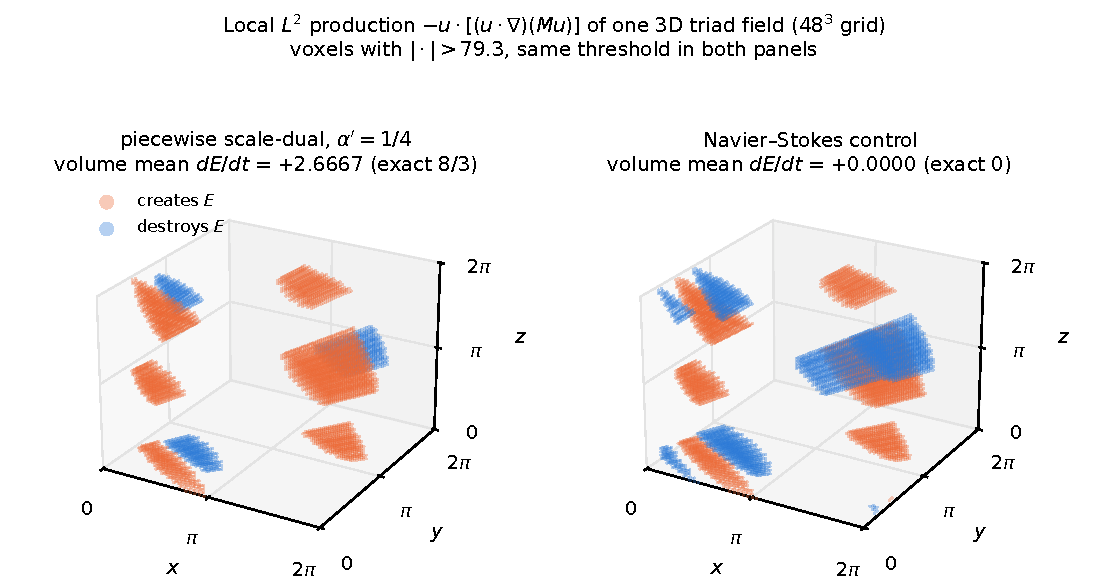
\includegraphics[width=\textwidth]{fig2_v2_energy_production_density_3d.pdf}
\caption{Local $L^2$ production density on $\mathbb{T}^3$ for one exact solenoidal triad at $\alpha'=1/4$, recomputed from the model on a $48^3$ grid. Orange voxels create kinetic energy and blue voxels destroy it; both panels use the same threshold, the $93$rd percentile of $|\cdot|$ for the scale-dual field. Left: piecewise scale-dual model, volume mean $+8/3$. Right: Navier--Stokes control on the same field, volume mean $0$.}
\label{fig:density}
\end{figure}

\subsection{Pseudospectral Galerkin ensemble}
\label{sec:dns}
\paragraph{Method.} The solver is a $2/3$-dealiased Fourier--Galerkin discretization of~\eqref{eq:model}, advanced with RK4 and an exact viscous integrating factor, on $N^3$ grids (\path{scripts/three_breakthroughs/paper_b_v2_experiment.py}). Initial data are random-phase solenoidal fields with spectrum $\propto k^4e^{-2(k/4)^2}$, normalized to energy $E_0$. The pre-registered ensemble uses $N=32$, $dt=0.005$, $t\le3$, ten seeds, the three models, $\alpha'\in\{1/4,1/16,1/25\}$ and $\nu\in\{0,1/400,1/100\}$, at $E_0=1/2$. Convergence checks at the paper's $(\alpha',\nu)$ use $N=64$ (zero-padded, identical initial data) and $dt/2$. A 0.5-time-unit smoke run of one seed at $E_0=1/2$ showed $E$ decreasing. Before any ensemble result existed, we therefore added an amplitude scan $E_0\in\{2,8,32\}$ (5 seeds) at the paper's $(\alpha',\nu)$, with convergence checks at $E_0=32$. The amendment is recorded in the script's docstring. In total there are 299 runs (13{,}257\,s wall time on 7 processes). One caveat on ``pre-registered'': the criteria, the controls and the amendment were all fixed in that docstring before the runs they govern, but the script was untracked in git at the time, so the ordering rests on the author's record and on file timestamps (the script was last written at 08:24:53 and the results JSON at 12:12:06, after a 13{,}257\,s run that therefore began around 08:31), not on a commit predating the run.

\paragraph{Code validation.} On the exact fields of A1 and A2, the float rates agree with the exact rationals $0$, $6/5$, $32/15$ and $6/13$ to $1.1\times10^{-15}$ at $N=16$ and $32$.

\paragraph{Ensemble ($N=32$, $E_0=1/2$, ten seeds; mean $\pm$ s.d.\ of $\max_{t\le3}E/E_0$).}
\begin{center}\footnotesize
\begin{tabular}{llccc}
\toprule
model & $\alpha'$ & $\nu=0$ & $\nu=1/400$ & $\nu=1/100$ \\
\midrule
Navier--Stokes & -- & $1.0000$ (drift $7.5\times10^{-10}$) & $1$ & $1$ \\
piecewise & $1/4$ & $1.459\pm0.022$ & $1$ & $1$ \\
 & $1/16$ & $2.892\pm0.034$ & $1.396\pm0.018$ & $1$ \\
 & $1/25$ & $2.722\pm0.021$ & $1.361\pm0.011$ & $1$ \\
smooth (ML-$\alpha$) & $1/4$ & $1.249\pm0.012$ & $1$ & $1$ \\
 & $1/16$ & $1.814\pm0.018$ & $1$ & $1$ \\
 & $1/25$ & $1.865\pm0.017$ & $1.007\pm0.006$ (8/10 seeds $>1$) & $1$ \\
\bottomrule
\end{tabular}
\end{center}
An entry $1$ means $E$ never exceeded $E_0$ (its maximum is the initial value). In every inviscid model run $Q$ was conserved to $|Q/Q_0-1|\le9.5\times10^{-11}$; the bound over the ensemble group alone is $8.7\times10^{-12}$, and the looser figure comes from the inviscid $N=64$ piecewise run (the triad evolution gives $4.3\times10^{-12}$). In every viscous model run $Q$ never increased (largest increase $0$). In every model run $\max_t\alpha'\Eff/Q_0\le0.9967\le1$, as Theorem~\ref{thm:ceiling} requires. The Galerkin bound $E\le\max(1,\alpha'N_{\max}^2)\,Q$ held in all runs. Figure~\ref{fig:traj} shows the trajectories in $(E/E_0,Q/Q_0,\alpha'\Eff/Q_0)$ space, and Fig.~\ref{fig:series}(a,b) the ensemble time series at $\alpha'=1/25$.

\paragraph{Exact triad field, evolved ($\alpha'=1/4$, $N=32$, $dt=0.002$, $t\le2$).} $\max_tE/E_0=2.511$ for piecewise and $1.539$ for smooth when inviscid ($Q$ conserved to $4.3\times10^{-12}$). At $\nu=1/100$ they are $1.510$ and $1.138$, both at $t\approx1.22$. Navier--Stokes stays at $1$.

\paragraph{Resolution dependence (inviscid, piecewise, $\alpha'=1/25$, seed 0).} $\max_tE/E_0=2.707$ at $N=32$ and $8.396$ at $N=64$. Energy growth is a transfer of $Q$-conserving content to subgrid modes, whose number grows with $N$ (Section~\ref{sec:directions}, item~4).

\begin{figure}[htbp]
\centering
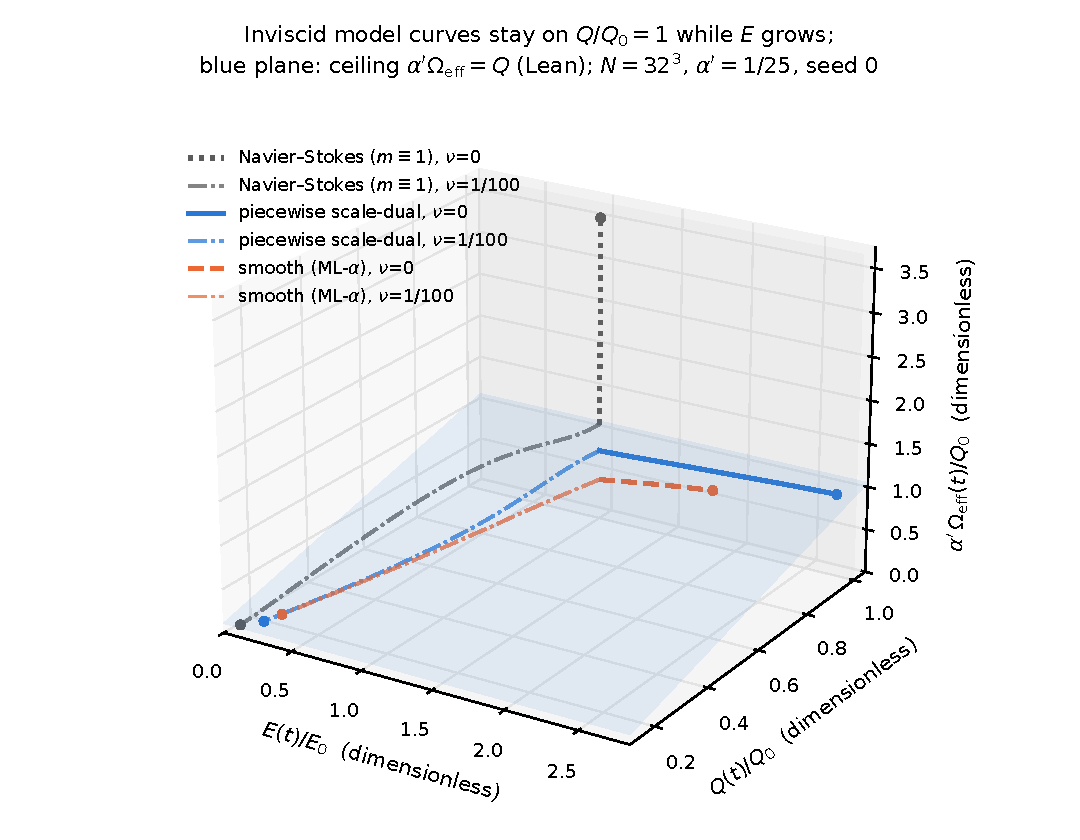
\includegraphics[width=0.82\textwidth]{fig1_v2_invariant_trajectories_3d.pdf}
\caption{Trajectories of seed~0 ($N=32^3$, $\alpha'=1/25$, $E_0=1/2$, $t\le3$) in the space of kinetic energy $E/E_0$, invariant $Q/Q_0$ and rescaled effective enstrophy $\alpha'\Eff/Q_0$. All quantities are dimensionless ratios. Inviscid model curves (solid, dashed) stay on the plane $Q/Q_0=1$ (grey) while $E/E_0$ rises to $\approx2.7$ (piecewise) and $\approx1.8$ (smooth). The inviscid Navier--Stokes curve (dotted) stays on $E/E_0=1$, and its $\alpha'\Omega/E_0$ rises to $3.6$, above the ceiling. The translucent blue plane is the Lean ceiling $\alpha'\Eff=Q$. Model curves never cross it. Dash-dot curves: $\nu=1/100$. Dots mark $t=3$.}
\label{fig:traj}
\end{figure}

\begin{figure}[htbp]
\centering
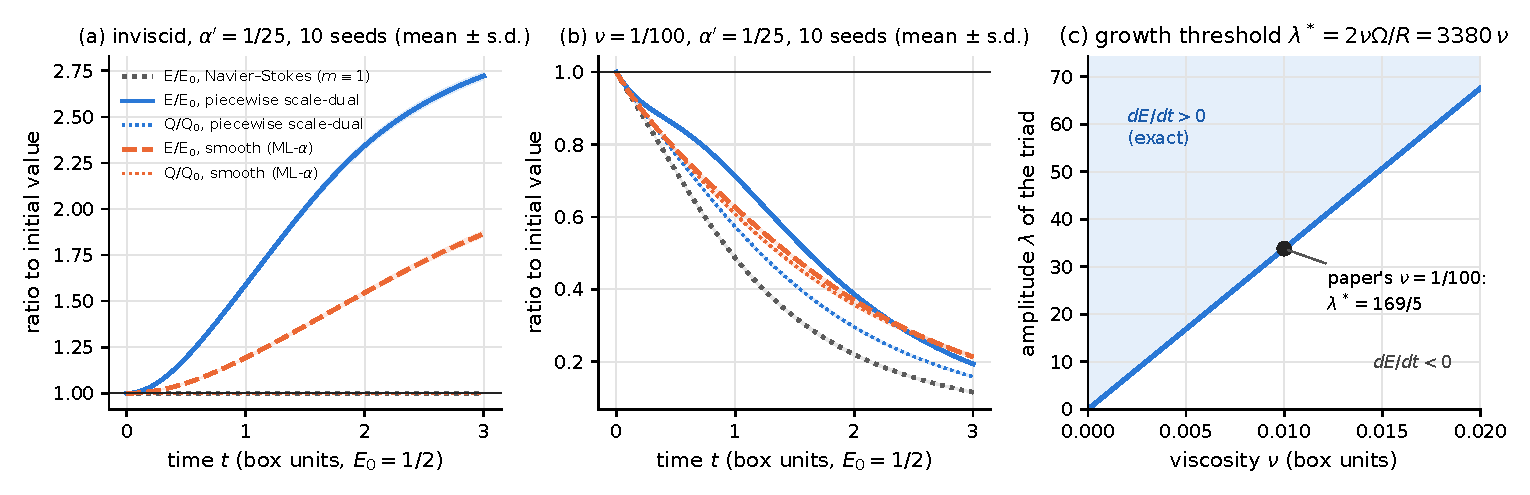
\includegraphics[width=\textwidth]{fig3_v2_energy_vs_Q_and_threshold.pdf}
\caption{(a,b) $E/E_0$ (thick) and $Q/Q_0$ (thin dotted) against time, mean $\pm$ one standard deviation over 10 seeds ($N=32^3$, $\alpha'=1/25$, $E_0=1/2$). In (a) the inviscid $Q/Q_0$ curves coincide with the line $1$. (c) Exact growth threshold of the $\alpha'=1/25$ triad of Section~\ref{sec:exact}: $dE/dt>0$ exactly when the amplitude exceeds $\lambda^*(\nu)=3380\,\nu$; edition~1's $\nu=1/100$ gives $\lambda^*=169/5$ (Lean \leanc{growth_threshold_iff}).}
\label{fig:series}
\end{figure}

\subsection{Controls}
\label{sec:controls}
We fixed the controls before running the model numbers. Both sets passed (\path{summary.positive_controls.passed} and \path{summary.negative_controls.passed} in the results file).
\begin{center}\footnotesize
\begin{tabularx}{\textwidth}{@{}l X >{\raggedright\arraybackslash}p{0.27\textwidth}@{}}
\toprule
type & check & observed \\
\midrule
positive & exact NS triads (A1, A2): $dE/dt=dQ/dt=0$ & $0$, $0$ \\
positive & exact sweeps: NS triads with $dE/dt\ne0$; constant-weight triads with $dE/dt\ne0$ & $0$; $0$ \\
positive & float rates equal the exact rationals & max error $1.1\times10^{-15}$ \\
positive & inviscid dealiased NS: $\max|E/E_0-1|$ over 10 seeds (RK4 time error) & $7.5\times10^{-10}$ \\
positive & Lean ceiling: $\max\alpha'\Eff/Q_0$ over all model runs; $\max(\alpha'\Eff-Q)/Q_0$ & $0.9967$; $-0.0013$ \\
negative & exact NS field with one non-solenoidal mode ($k\cdot\hat u_k=1$) & $dE/dt=-2\ne0$ \\
negative & aliased (not dealiased) inviscid NS, seed 0: $\max|E/E_0-1|$ & $4.6$ at the last finite sample $t=0.90$, then overflow between $t=0.90$ and $t=0.95$; dealiased: $7.3\times10^{-10}$ \\
negative & NS runs whose true enstrophy exceeds $E_0/\alpha'$ (no ceiling without the filter; Lean \leanc{ns_enstrophy_not_capped}) & 30 of 30 \\
\bottomrule
\end{tabularx}
\end{center}
The last line is also the empirical form of item~2 in Section~\ref{sec:corrections}. For the scale-dual models the true enstrophy is not capped either: $\max_t\alpha'\Omega/E_0$ reached $1.1$--$17$ across the ensemble, while $\alpha'\Eff/Q_0$ stayed below $1$.

\subsection{Outcome}
\label{sec:outcome}
\paragraph{Edition-2 claim.} The claim is: ``$E$ is not a Lyapunov functional of the scale-dual model; $Q$ is.'' The pre-registered falsifiers were any exact divergence-free field with $dQ/dt\ne0$, or no non-constant-weight triad with $dE/dt\ne0$. Neither occurred: there were $0$ fields with $dQ/dt\ne0$ out of $59{,}780$ exact evaluations (A1, A2, and both sweeps for all three models), and $12{,}200$ ($\alpha'=1/25$) and $972$ ($\alpha'=1/4$) piecewise triads move $L^2$ energy. \textbf{Not falsified.}

\paragraph{Edition-1 Theorem~2.5, $E(t)\le E_0$, at $(\alpha',\nu)=(1/25,1/100)$.} The pre-registered refutation needs a positive exact rate for some amplitude (A2: yes, for $\lambda>169/5$). It also needs, in the DNS, $\max_tE/E_0-1$ above $10\times$ the NS control's excess (floored at $10^{-12}$), persisting under $N\to64$ and $dt\to dt/2$. Results (Fig.~\ref{fig:amplitude}):
\begin{itemize}
  \item $E_0=1/2$: $E(t)\le E_0$ in all 10 seeds and in the $N=64$ and $dt/2$ reruns, for both models. At this amplitude only instantaneous growth (the exact triads) is shown.
  \item $E_0=2$ and $8$: the piecewise model exceeds $E_0$ in 5/5 seeds ($\max E/E_0=1.034\pm0.006$ and $1.356\pm0.008$). The smooth model exceeds it at $E_0=8$ in 4/5 seeds (up to $1.012$).
  \item $E_0=32$: piecewise $1.767\pm0.015$, smooth $1.247\pm0.014$ (5/5 seeds each). For seeds 0--2, halving $dt$ changes $\max E/E_0$ by $3.5\times10^{-7}$ (piecewise) and $\le3.8\times10^{-8}$ (smooth). $N=64$ \emph{increases} it to $2.96$--$3.00$ (piecewise) and $1.50$--$1.52$ (smooth). The NS control stays at exactly $1$.
\end{itemize}
\textbf{Verdict: refuted for the piecewise model at $E_0=32$} by the pre-registered criterion, and also exceeded for the smooth (ML-$\alpha$) model. The excess is robust to the time step but its magnitude is not converged in $N$. It increases with resolution, consistent with energy transfer to subgrid modes permitted by $Q$-conservation. We therefore claim that $E(t)>E_0$ occurs and persists under refinement at the paper's parameters; we do not claim a converged value of $\sup_tE/E_0$.

\begin{figure}[htbp]
\centering
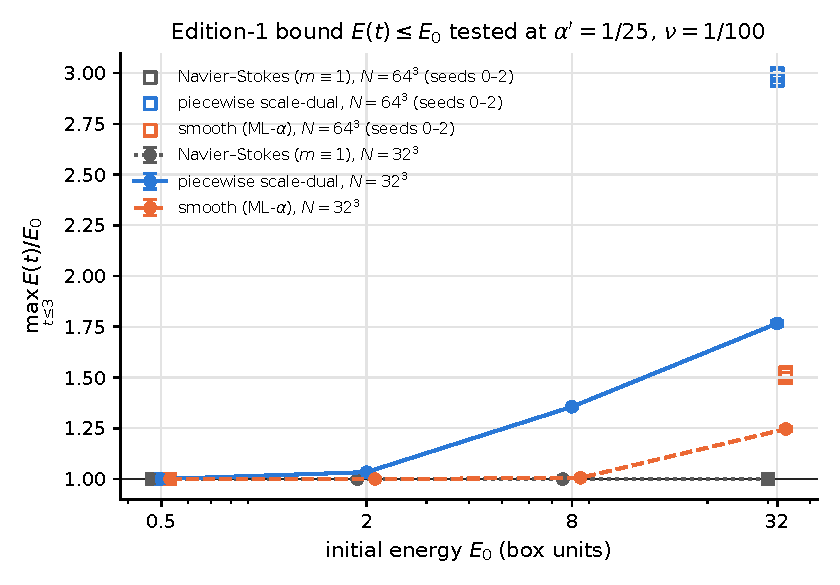
\includegraphics[width=0.66\textwidth]{fig4_v2_amplitude_scan.pdf}
\caption{Test of edition~1's $E(t)\le E_0$ at its own $\alpha'=1/25$, $\nu=1/100$. The plot shows $\max_{t\le3}E/E_0$ against the initial energy $E_0$. Filled markers: $N=32^3$ mean $\pm$ s.d.\ (10 seeds at $E_0=1/2$, 5 seeds otherwise), with individual seeds as faint dots. Open squares: $N=64^3$ reruns of seeds 0--2 at $E_0=1/2$ and $32$. Navier--Stokes stays at $1$.}
\label{fig:amplitude}
\end{figure}

\section{Retained arithmetic from edition 1, relabelled}
\label{sec:retained}
\paragraph{Illustrative radii-polynomial arithmetic (edition~1, Theorem~2.1).} Take the \emph{hypothetical} bounds $Y_0=1/10000$, $Z_0=7/20$, $Z_1=1/200$, $Z_{\mathrm{tail}}=1/200$, $Z_2=12$ and $r_*=1/1000$. Then $Z_0+Z_2r_*=181/500$, $Z_0+Z_1+Z_{\mathrm{tail}}+Z_2r_*=93/250$, and $P(r_*)=Y_0+(Z_0+Z_1+Z_{\mathrm{tail}}-1)r_*+Z_2r_*^2=-33/62500<0$. Replacing $Z_{\mathrm{tail}}$ by $1/800$ gives $1473/4000$ and $-2127/4000000$. These identities are proved over $\mathbb{Q}$ in \lean{P2_T1}. If such bounds were \emph{derived} for an actual approximate solution, the radii-polynomial theorem~\cite{DayLessard2007,Nakao2019} would give a zero of $F$ within $r_*$. No such derivation exists here; Section~\ref{sec:directions}, item~3 describes what one would require. The former ``hurricane'' number $443/1000$ is the sum $21/50+3/500+1/500+15/1000$ and refers to no equation.

\section{Scope and limitations}
\label{sec:scope}
\begin{itemize}
  \item The Lean theorems concern finite Galerkin truncations with an abstract skew tensor. They do not formalize $\mathbb{T}^3$, the Fourier basis or the Leray projector. That the Fourier--Galerkin truncation of~\eqref{eq:model} has this form is standard but not machine-checked. Passing to the limit $N\to\infty$ (existence and regularity of solutions) is not addressed.
  \item The ceiling $\Eff\le E_0/\alpha'$ bounds a model-internal quantity. $\Eff=\tfrac12\|\nabla Mu\|^2$ is not the enstrophy of $u$, and no statement about blow-up or regularity of~\eqref{eq:model} or of Navier--Stokes follows from it. In our runs the true enstrophy is not bounded by $E_0/\alpha'$ (Section~\ref{sec:controls}).
  \item The DNS are $32^3$ (and $64^3$ checks) on a $2\pi$-periodic box over $t\le3$, with one random-phase spectral shape. They are not low-Reynolds-number runs, and we do not claim they are: at the refutation amplitude $E_0=32$ with $\nu=1/100$, $u_{\mathrm{rms}}\approx4.6$ and $L\approx1.6$ give a Reynolds number of order $7\times10^2$ and a Kolmogorov wavenumber of order $10^2$, far above $k_{\max}=10$ ($N=32$) or $21$ ($N=64$). The $E_0=32$ runs are strongly under-resolved, which is consistent with doubling $N$ raising $\max E/E_0$ from about $1.77$ to about $3.0$ (two resolutions cannot establish that the under-resolution is the cause); the occurrence and persistence of $E>E_0$ is what we claim from them, never a converged value. ``Units'' throughout are box units ($L=2\pi$, unit density). They test the energy budget. They are not turbulence simulations, and inviscid runs of a truncated system thermalize.
  \item The sign of $dE/dt$ is cubic in $u$ and flips under $u\to-u$. The ``$dE/dt>0$'' counts in the sweep are therefore not growth probabilities; the relevant count is the number of triads that move $L^2$ energy at all.
  \item No PARI/GP or Sage installation was available on the build host. All exact arithmetic here is integer/rational arithmetic in Python (\texttt{fractions}) and in the Lean kernel (\texttt{norm\_num}); it involves no number theory.
  \item This edition has not been reviewed by anyone outside the author's own checks.
\end{itemize}

\section{Research directions}
\label{sec:directions}
\begin{enumerate}
  \item \emph{Global regularity for the piecewise symbol.} By $m_{\mathrm{ML}}\le m_{\mathrm{pw}}\le2m_{\mathrm{ML}}$, the invariant $Q$ is equivalent, within a factor~$2$, to the ML-$\alpha$ energy $\tfrac12\langle u,\tilde u\rangle=\tfrac12(\|\tilde u\|^2+\alpha'\|\nabla\tilde u\|^2)$, $\tilde u=(I-\alpha'\Delta)^{-1}u$. Does the ML-$\alpha$ well-posedness argument~\cite{ILT2006} carry over despite the kink of $m_{\mathrm{pw}}$ at $k_*$? This is open until proved.
  \item \emph{Dynamical test of ``zero inertial distortion''.} At $64^3$ and above, compare resolved-band trajectories and spectra of the piecewise model and ML-$\alpha$ against a Navier--Stokes reference at the same $\nu$. The kink may instead cause Gibbs-type artefacts.
  \item \emph{A genuine computer-assisted proof.} Validate a steady state of Kolmogorov-forced ML-$\alpha$ or scale-dual flow on $\mathbb{T}^3$. This needs a computed $\bar u$, interval-arithmetic $Y_0,Z_0,Z_1,Z_2$, and a tail bound that keeps the one-derivative loss and $\|\bar u\|$ explicit. Only the final rational inequalities would go to Lean. Chen and Hou~\cite{ChenHou2022a,ChenHou2022b} show what such a fluid CAP involves.
  \item \emph{Energy transfer to subgrid scales.} In a truncation $|k|\le N$ with $N>k_*$, $E\le\alpha'N^2Q$ (checked in every run). Measure how $\sup_tE/E_0$ scales with $N$: Section~\ref{sec:dns} gives the first two points.
  \item \emph{Spectral scaling beyond $k_*$.} Measure the piecewise model's spectrum and compare it with the published Leray-$\alpha$ and ML-$\alpha$ predictions. This would replace the deleted ``$-84/125$''.
\end{enumerate}

\section*{Reproducibility}
From the repository root:
\begin{itemize}
  \item \path{.venv/bin/python scripts/three_breakthroughs/paper_b_v2_experiment.py} (writes \path{papers/three_breakthroughs/paper_b/paper_b_v2_results.json});
  \item \path{.venv/bin/python scripts/three_breakthroughs/paper_b_v2_figures.py} (writes the figure PDFs and \path{paper_b_v2_fig2_values.json});
  \item \path{.venv/bin/python -m anse.formal.lean_runner formal/ANSE/PaperB_EnergyBudget.lean}, and the same for \path{formal/ANSE/PaperB_ScaleDualEd2.lean};
  \item \path{.venv/bin/python -m pytest tests/test_paper_b_v2_experiment.py -q -p no:cacheprovider}.
\end{itemize}
The experiment's design, controls and falsification criteria are fixed in the docstring of the experiment script. That includes the one amendment made before any ensemble result existed.

One naming warning for anyone reading the bundle: the figure \emph{file} names do not follow the figure numbers in this PDF. Figure~\ref{fig:symbols} is \path{fig5_v2_symbols.pdf}, Figure~\ref{fig:density} is \path{fig2_v2_energy_production_density_3d.pdf}, Figure~\ref{fig:traj} is \path{fig1_v2_invariant_trajectories_3d.pdf}, Figure~\ref{fig:series} is \path{fig3_v2_energy_vs_Q_and_threshold.pdf} and Figure~\ref{fig:amplitude} is \path{fig4_v2_amplitude_scan.pdf}. The numbering inside the document is consistent; only the file names are historical.

\appendix
\section{An algebraic identity (edition 1, Theorem 2.4)}
\label{app:sym2}
If $u_{n+2}=au_{n+1}+bu_n$ and $v_{n+2}=av_{n+1}+bv_n$, then $w_n=u_nv_n$ satisfies $w_{n+3}=(a^2+b)w_{n+2}+b(a^2+b)w_{n+1}-b^3w_n$. This is the first conjunct of \lean{P2_T4}, proved by \texttt{ring}. No physical interpretation is claimed.

\begin{thebibliography}{10}
\bibitem{ChenHou2022a} J.~Chen and T.~Y. Hou, ``Stable nearly self-similar blowup of the 2D Boussinesq and 3D Euler equations with smooth data I: Analysis,'' \texttt{arXiv:2210.07191}.
\bibitem{ChenHou2022b} J.~Chen and T.~Y. Hou, ``Stable nearly self-similar blowup of the 2D Boussinesq and 3D Euler equations with smooth data II: Rigorous numerics,'' \texttt{arXiv:2305.05660}.
\bibitem{Cheskidov2005} A.~Cheskidov, D.~D. Holm, E.~Olson, and E.~S. Titi, ``On a Leray-$\alpha$ model of turbulence,'' \emph{Proc.\ R.\ Soc.\ A}, vol.~461, pp.~629--649, 2005.
\bibitem{DayLessard2007} S.~Day, J.-P. Lessard, and K.~Mischaikow, ``Validated continuation for equilibria of PDEs,'' \emph{SIAM J.\ Numer.\ Anal.}, vol.~45, no.~4, pp.~1398--1424, 2007.
\bibitem{FoiasHolmTiti2001} C.~Foias, D.~D. Holm, and E.~S. Titi, ``The Navier--Stokes-alpha model of fluid turbulence,'' \emph{Physica D}, vol.~152--153, pp.~505--519, 2001.
\bibitem{ILT2006} A.~A. Ilyin, E.~M. Lunasin, and E.~S. Titi, ``A modified-Leray-$\alpha$ subgrid scale model of turbulence,'' \emph{Nonlinearity}, vol.~19, no.~4, pp.~879--897, 2006. DOI: 10.1088/0951-7715/19/4/006.
\bibitem{Nakao2019} M.~T. Nakao, M.~Plum, and Y.~Watanabe, \emph{Numerical Verification Methods and Computer-Assisted Proofs for Partial Differential Equations}. Springer, 2019.
\end{thebibliography}

\end{document}
